\documentclass[12pt]{article}
\usepackage{sbc-template}
\usepackage{graphicx,url}
\usepackage[brazil]{babel}
\usepackage[utf8]{inputenc}
\usepackage{amssymb}
\usepackage{amsmath}
\usepackage{comment}
\usepackage[linesnumbered,ruled,vlined,portuguese]{algorithm2e}
\usepackage{subfigure}

\sloppy

\title{Otimização Matemática Através de Algoritmos Genéticos}

\author{Fernando Concatto\inst{1}}

\address{Bacharelado em Ciência da Computação -- Universidade do Vale do Itajaí (UNIVALI) \\
  Caixa Postal 360 -- CEP 88302-202 -- Itajaí -- SC -- Brasil
  \email{fernandoconcatto@edu.univali.br}
}

\begin{document}

\maketitle

\begin{abstract}
  Problems involving mathematical optimization are ubiquitous in many fields of science. Since many of them exhibit elevated computational complexity, several approximation methods have been developed to solve such problems. This paper describes the notion of genetic algorithms, which employs concepts of evolution and natural selection to approximate the highest or lowest value of a function, improving candidate solutions with the passing of generations.
\end{abstract}

\begin{resumo}
  Problemas envolvendo otimização matemática são ubíquos em diversas áreas da ciência. Como grande parte desses problemas apresenta uma dificuldade computacional muito elevada, diversos métodos aproximados para resolvê-los foram desenvolvidos. Este trabalho descreve os algoritmos genéticos, que aplicam conceitos de evolução e seleção natural para aproximar o ponto máximo ou mínimo de uma função, aprimorando soluções candidatas com o decorrer das gerações.
\end{resumo}


\section{Introdução} \label{sec:intro}

O estudo de problemas e suas soluções compõe o cerne do campo da Ciência da Computação. Para efetuar a solução dos problemas, uma sequência finita de operações deve ser desenvolvida; tais sequências são conhecidas como algoritmos. Problemas abordados por cientistas da computação possuem uma enorme gama de formulações e dificuldades, alguns tão complexos que demandam mais do que o tempo de vida um ser humano para serem resolvidos. Um exemplo de problema com esta característica é o Problema do Caixeiro Viajante, definido da seguinte forma: dado um conjunto de $n$ cidades e as distâncias entre elas, qual a rota mais curta que parte de uma cidade, passa por todas as outras e retorna para a cidade inicial? Como existem $(n-1)!/2$ rotas possíveis, descobrir a menor rota entre 30 cidades através de um algoritmo exato requer muito mais do que um milhão de anos de processamento \cite{MacGregor2011}.

Para tratar de problemas com esse nível de complexidade, métodos \textbf{heurísticos} são usualmente aplicados. Algoritmos heurísticos são potencialmente capazes de resolver problemas complexos em pouquíssimo tempo, porém não garantem que a solução exata seja encontrada, fornecendo apenas aproximações, que geralmente são suficientes para grande parte dos problemas reais \cite{Kokash2005}. Exemplos de algoritmos heurísticos para problemas específicos incluem o algoritmo de Christofides para o problema do Caixeiro Viajante \cite{Christofides1976}, mencionado anteriormente, e o algoritmo de Kernighan-Lin para particionamento de grafos \cite{Kernighan1970}.

Entretanto, a categoria de algoritmos heurísticos que mais recebeu atenção da comunidade científica é a que envolve a resolução de \textbf{problemas de otimização}, caracterizada pela busca por um valor $x \in X$ que maximiza ou minimiza uma função $f: X \rightarrow \mathbb{R}$, geralmente chamada de \textbf{função objetivo}. Grande parte dos problemas, tanto inéditos quanto clássicos, podem ser formulados como problemas de otimização, incluindo o Problema do Caixeiro Viajante, onde a função objetivo pode ser descrita por:

\begin{equation} \label{eq:tsp}
    \mathop{\boldsymbol\min} f(x) = \sum_{i = 1}^{n - 1} d(x_{i}, x_{i + 1}) + d(x_{n}, x_{1})
\end{equation}

\noindent onde $x$ é o conjunto que descreve a rota candidata e $d(x_{i}, x_{j})$ é a distância entre as cidades $x_{i}$ e $x_{j}$. Desta forma, um algoritmo pode mover-se iterativamente pelo \textit{espaço de busca}, que contém todas as rotas possíveis, buscando um conjunto $x$ que minimize a função $f(x)$. Porém, este espaço de busca (assim como de vários outros problemas) apresenta uma quantidade excessivamente grande de elementos, exigindo então a aplicação de métodos heurísticos.

Problemas de otimização envolvem várias disciplinas, como pesquisa operacional, economia e as ciências naturais. A análise numérica é um dos campos com maior influência no estudo dos problemas de otimização, devido ao foco em métodos iterativos e aproximados, como o Método de Newton, através do qual é possível encontrar máximos ou mínimos locais se for aplicado à primeira derivada de uma função. Outro método capaz de encontrar pontos críticos é o Método dos Gradientes, que guia uma solução candidata para um ponto mínimo ou máximo a partir do gradiente de uma função. Este método é frequentemente aplicado em Redes Neurais Artificiais para guiar a aprendizagem da rede \cite{Haykin1998}.

Este trabalho busca descrever o método heurístico conhecido como Algoritmo Genético, que utiliza conceitos da biologia evolucionária para otimizar uma função objetivo. Para este fim, a seção \ref{sec:introevolution} introduz alguns conceitos relativos à evolução por seleção natural; por sua vez, a seção \ref{sec:algorithm} apresenta a construção do Algoritmo Genético, descrevendo sua estrutura fundamental; já a seção \ref{sec:geneticoperators} define os operadores genéticos de seleção, mutação e reprodução; por fim, a seção \ref{sec:conclusions} apresenta uma breve discussão sobre o método, concluindo o trabalho.

\section{O processo evolucionário} \label{sec:introevolution}

O conceito de evolução de organismos é bastante antigo, datando da época dos filósofos gregos pré-socráticos \cite{Hull1967}. A noção de seleção natural  foi desenvolvida por Charles Darwin, com a publicação de seu livro ``A Origem das Espécies'', de 1859. Nele, Darwin propõe que populações evoluem ao longo de gerações através de um processo de seleção que favorece organismos com aptidão alta, medida através do sucesso reprodutivo. Indivíduos aptos produzem descendentes, que herdam boa parte de suas características (genes), e portanto também tendem a possuir elevado sucesso reprodutivo.

Desta maneira, a cada geração, os melhores indivíduos da população são escolhidos naturalmente para reprodução, passando adiante suas características, enquanto os indivíduos menos aptos tendem a desaparecer. Assim, a próxima geração será composta tanto pelos indivíduos aptos sobreviventes quanto por seus descendentes, ambos possuindo uma aptidão média superior à geração passada. Algoritmos genéticos buscam simular esse processo, modelando os mecanismos da natureza de forma computacional, com o intuito de otimizar uma função objetivo.

\section{Os algoritmos genéticos} \label{sec:algorithm}

Algoritmos genéticos são classificados como meta-heurísticas, ou seja, são independentes do problema sendo resolvido. Qualquer problema que possa ser formulado por uma função objetivo pode ser solucionado por um algoritmo genético. Adicionalmente, algoritmos genéticos não possuem uma definição absolutamente rigorosa quanto aos detalhes dos procedimentos realizados; ao invés disso, são caracterizados pela existência de alguns elementos fundamentais \cite{Mitchell1998}, vistos adiante.

\subsection{Modelagem de cromossomos} \label{sec:chromosomes}

O primeiro destes elementos é a especificação dos \textbf{cromossomos}, que caracterizam os indivíduos da população. Cromossomos representam as soluções do problema, e a maneira como eles são codificados é um dos principais fatores envolvidos no desenvolvimento de um algoritmo genético bem sucedido.

Historicamente, o método mais utilizado para modelar cromossomos foi a codificação por cadeias de bits, porém outros métodos podem ser empregados, especialmente para problemas mais complexos \cite{Mitchell1998}. Por exemplo, para o Problema do Caixeiro Viajante, apresentado na introdução deste trabalho, um cromossomo pode ser constituído pela sequência de cidades que especifica a rota a ser tomada.

\subsection{Função de aptidão} \label{sec:fitnessfunction}

O segundo elemento fundamental de um algoritmo genético é a função objetivo propriamente dita, denominada \textbf{função de aptidão} nesse contexto. A função de aptidão é responsável por avaliar a qualidade dos indivíduos, e é utilizada para selecioná-los para reprodução. Geralmente, devido ao caráter biológico, a função de aptidão é maximizada; caso a intenção seja a minimizar a função, é possível utilizar o inverso multiplicativo da função, definido como $1 / f(x)$.

\subsection{Operadores genéticos} \label{sec:operatorsbrief}

Por fim, os elementos que concluem a base dos algoritmos genéticos são os \textbf{operadores genéticos}. Os principais operadores são a \textbf{seleção}, que utiliza a função de aptidão para selecionar indivíduos; a \textbf{reprodução} (ou cruzamento), que combina dois indivíduos para produzir um descendente; e a \textbf{mutação}, que aleatoriamente altera um ou mais genes do cromossomo. Estes operadores e as técnicas utilizadas para implementá-los são detalhados na seção \ref{sec:geneticoperators}.

\subsection{Evolução} \label{sec:evolution}

Com todos estes elementos definidos, resta especificar o procedimento de evolução propriamente dito. Este é um dos segmentos mais flexíveis de um algoritmo genético. Muitas variações existem para a implementação deste processo, algumas extremamente complexas e outras razoavelmente simples. Um exemplo básico, porém bastante eficiente para grande parte dos problemas, é apresentado adiante.

Inicialmente, uma população de $n$ indivíduos é estabelecida, com seus cromossomos construídos aleatoriamente ou através de outros métodos.
Como a otimização por algoritmos genéticos é um processo iterativo, os seguintes passos são repetidos até que uma solução satisfatória seja encontrada. A primeira etapa consiste no cálculo da aptidão de cada indivíduo $x$ da população, através da função de aptidão $f(x)$. Na sequência, uma nova geração de indivíduos é produzida a partir da aplicação dos operadores genéticos.

Dois indivíduos são selecionados através do operador de seleção, que favorece indivíduos mais aptos. Então, um ou mais filhos são concebidos pelo operador de reprodução, herdando as características de seus pais. Cada filho passa pelo operador de mutação, possivelmente sofrendo alterações genéticas em seu cromossomo. Este procedimento é repetido até que uma quantidade suficiente de filhos seja gerada.

Por fim, a população de indivíduos que foram selecionados para reprodução é unida com a população de filhos concebidos, formando uma nova população de tamanho $n$. Este processo é repetido até que alguma determinada condição de término seja atingida. O algoritmo \ref{alg:geneticalgorithm} formaliza essa sequência de passos por meio de uma representação em pseudocódigo.

\begin{algorithm}[ht]
  \small
  \DontPrintSemicolon
  \caption{Algoritmo genético básico}
  \label{alg:geneticalgorithm}
  \SetKwInOut{Input}{Entrada}
  \SetKwInOut{Output}{Saída}
  \Input{Tamanho da população ($n$), chance de mutação ($m$)}
  \Output{Indivíduos evoluídos}
  \BlankLine
  $populacao \leftarrow gerarPopulacaoInicial(n)$ \;
  \BlankLine
  \Repeat{condição de parada não for atingida}{
      \ForEach{individuo $\in$ populacao}{
        $individuo.aptidao \leftarrow calcularAptidao(individuo)$ \;
      }
      $filhos \leftarrow \emptyset$ \;
      \BlankLine
      \While{quantidade de filhos for insuficiente}{
        $pais \leftarrow selecionar(populacao)$ \;
        $filho \leftarrow reproduzir(pais)$ \;
        \BlankLine
        \If{aleatorio() $<$ m}{
            $aplicarMutacao(filho)$ \;
        }
        $filhos \leftarrow filhos \cup \{filho\}$ \;
      }
      $populacao \leftarrow combinar(populacao, filhos)$ \;
  }
  \BlankLine
  \Return{populacao}
\end{algorithm}

Ao término deste algoritmo, caso não haja nenhuma falha na definição dos cromossomos, função de aptidão ou operadores genéticos, a população final possuirá uma qualidade consideravelmente superior à inicial, dependendo da topologia do espaço de busca do problema e da quantidade de gerações decorridas. Entretanto, por se tratar de um algoritmo heurístico, não há garantia de que soluções ótimas serão encontradas, mesmo com uma grande quantidade de gerações.

\section{Operadores genéticos} \label{sec:geneticoperators}

Os operadores genéticos constituem as técnicas utilizadas para guiar as soluções candidatas (indivíduos) em direção a estados cada vez mais próximos da solução ótima. Uma breve introdução aos operadores de seleção, reprodução e mutação foi realizada na seção \ref{sec:operatorsbrief}; esta seção é dedicada a apresentar com detalhes as particularidades de cada operador.

\subsection{Operador de seleção}

O operador de seleção é responsável por escolher indivíduos para reprodução. O método de seleção deve enfatizar indivíduos aptos, para que seus descendentes também sejam aptos. Entretanto, também deve haver uma baixa chance de selecionar indivíduos com pouca aptidão -- caso contrário, haverá pouca diversidade genética na população, dificultando ou até mesmo impedindo a evolução das soluções para um estado melhor \cite{Mitchell1998}.

Diversos métodos de seleção foram propostos por pesquisadores no campo. A seguir, as técnicas conhecidas como \textit{seleção por roleta} e \textit{seleção por torneio}, por serem amplamente utilizadas e razoavelmente simples.

\subsubsection{Seleção por roleta} \label{sec:roulette}

O método de seleção por roleta envolve a atribuição de uma chance de seleção para cada indivíduo proporcional à sua aptidão. Conceitualmente, este método constrói uma roleta onde cada casa corresponde indivíduo, com casas maiores para indivíduos mais aptos. Esta técnica é uma das mais antigas, datada das primeiras pesquisas sobre algoritmos genéticos, e ainda é frequentemente utilizada hoje em dia.

Para efetuar a seleção por roleta, o primeiro passo a ser realizado é somar a aptidão de todos os indivíduos da população. Na sequência, um número aleatório $r$ é escolhido, no intervalo de 0 até a soma calculada. Então, a sequência de indivíduos da população é percorrida, acumulando a aptidão de cada indivíduo visitado até que esse valor ultrapasse o número aleatório $r$. O último indivíduo visitado é escolhido para reprodução \cite{Mitchell1998}.

\subsubsection{Seleção por torneio} \label{sec:tournament}

A seleção por torneio foi desenvolvida um pouco depois da seleção por roleta, e apresenta uma complexidade computacional significativamente melhor. O método da roleta requer o somatório da aptidão dos indivíduos da população, que demanda uma quantidade de operações proporcional ao tamanho da população.

Na técnica da seleção por torneio, dois indivíduos são escolhidos da população de forma completamente aleatória. Então, um número é escolhido aleatoriamente no intervalo de 0 a 1. Se esse número for inferior a um parâmetro $k$ previamente definido, o indivíduo mais apto entre eles será escolhido para reprodução; caso contrário, o indivíduo menos apto é selecionado \cite{Mitchell1998}. Geralmente, valores próximos de 0.75 são escolhidos para o parâmetro $k$.

\subsection{Operador de reprodução} \label{sec:crossover}

O operador de reprodução é um dos aspectos mais marcantes dos algoritmos genéticos. Este operador é responsável por combinar os cromossomos dos indivíduos, produzindo filhos com características similares às dos seus pais. Na maior parte das vezes, um filho possuirá aptidão superior à de seus pais, mas também existe a possibilidade da criação de um filho com aptidão muito inferior. A probabilidade de conceber um filho mais apto que seus pais depende de diversos fatores, como a modelagem dos cromossomos, a complexidade do problema e do próprio operador de reprodução.

A técnica mais básica para efetuar a reprodução é o \textbf{cruzamento de ponto único}. Neste método, os genes de um dos pais são copiados para o cromossomo do filho até que um ponto previamente especificado (fixo ou aleatório) seja atingido. A partir desse ponto, os genes do outro pai passam a ser copiados, até que o cromossomo do filho esteja totalmente formado.

Entretanto, para cromossomos mais complexos com quantidade elevada de genes, a técnica de cruzamento de ponto único se mostra insuficiente; nestes casos, a maioria dos filhos apresenta aptidão inferior à de seus pais. Desta forma, outros métodos de reprodução foram desenvolvidos, como o \textbf{cruzamento de múltiplos pontos}, que é equivalente ao cruzamento de ponto único, porém com mais pontos de troca (geralmente dois); e o \textbf{cruzamento uniforme paramétrico}, onde a troca acontece a cada gene copiado, com chance igual a um parâmetro $p$ \cite{Mitchell1998}. A figura \ref{fig:crossover} apresenta uma demonstração gráfica destes três métodos.

\begin{figure}
    \centering
    \subfigure[Ponto único]{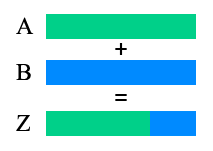
\includegraphics[width=4cm]{single.png}}
    \hspace{0.8cm}
    \subfigure[Múltiplos pontos]{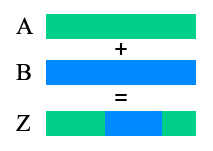
\includegraphics[width=4cm]{multiple.png}}
    \hspace{0.8cm}
    \subfigure[Uniforme]{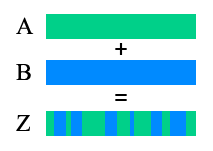
\includegraphics[width=4cm]{uniform.png}}
    \caption{Métodos de reprodução entre dois pais A e B, produzindo um filho Z.}
    \label{fig:crossover}
\end{figure}

\subsection{Operador de mutação} \label{sec:mutation}

O último dos operadores de um algoritmo genético é o operador de mutação. Sua tarefa consiste em elevar a variação genética da população, impedindo que genes fiquem fixados em valores distantes do ótimo; este fenômeno é conhecido como \textbf{ótimo local} no contexto da otimização matemática. Encontrar a solução ótima global evitando a fixação em ótimos locais é um problema extraordinariamente difícil, e o operador de mutação é uma das principais ferramentas utilizadas pelos algoritmos genéticos na resolução desse problema, juntamente com o operador de reprodução \cite{Mitchell1998}.

O operador de mutação deve gerar alguma perturbação no cromossomo de um indivíduo. Esta perturbação pode tomar diversas formas, sendo que as mais comuns envolvem a alteração de um ou mais genes do cromossomo para um valor diferente do atual. Para o caso de cadeias de bits, o gene escolhido para mutação pode ter seu bit invertido; para o caso de valores reais, um número aleatório pode ser somado ou subtraído ao valor do gene, ou o valor pode ser substituído por um número aleatório.

\section{Aplicações dos algoritmos genéticos} \label{sec:applications}

Por ser uma meta-heurística, o método de otimização por algoritmos genéticos encontra utilização em uma enorme gama de problemas. Pelo mesmo motivo, entretanto, os algoritmos genéticos não garantem que a solução ótima será encontrada, e portanto devem ser utilizados somente em problemas onde soluções aproximadas são admissíveis. Geralmente, problemas com essa característica apresentam espaços de busca extremamente extensos, como o Problema do Caixeiro Viajante, apresentado na seção \ref{sec:intro}. Alguns exemplos práticos são descritos adiante.

Um caso recente de aplicação de algoritmos genéticos ocorreu durante o evento Opção Profissional por Área (OPA) de 2016, organizado pela Universidade do Vale do Itajaí. O evento tem como público-alvo jovens que se encontram no processo de escolha de um curso superior. Para apresentar o curso de Ciência da Computação, os integrantes do Laboratório de Inteligência Aplicada desenvolveram um algoritmo genético que evolui imagens compostas por pixels aleatórios em direção a uma imagem real, desafiando os espectadores a descobrir qual era a imagem enquanto introduziam conceitos de inteligência artificial e complexidade computacional.

Outra aplicação de algoritmos genéticos, desta vez no cenário da análise de redes complexas, foi na detecção de comunidades, caracterizadas por grupos de indivíduos (também conhecidos como nodos ou vértices) fortemente conectados entre si. Neste contexto, os cromossomos representam possíveis divisões da rede em comunidades, e a função de aptidão calcula a qualidade da divisão, através de função de modularidade proposta por \cite{Newman2004} ou alguma variação da mesma. Por meio de experimentos, a eficiência dos algoritmos genéticos na detecção de comunidades foi evidenciada, superando diversos métodos similares tanto em qualidade quanto em desempenho \cite{Tasgin2007,Pizzuti2008}.

Algoritmos genéticos foram aplicados em muitos outros problemas com sucesso considerável. O trabalho de \cite{Ross1994} apresenta uma visão geral sobre esses problemas, incluindo a otimização de planejamento \textit{scheduling problem}, que consiste na organização de uma agenda, evitando conflitos espaciais e temporais, e também apresenta algumas aplicações no campo da engenharia, como no desenvolvimento de circuitos integrados, rotores de helicópteros, controle de braços robóticos, entre outras aplicações.

\section{Discussão e conclusões} \label{sec:conclusions}

Neste trabalho, a técnica de otimização matemática por algoritmos genéticos foi examinada. As características fundamentais de um algoritmo genético foram apresentadas, juntamente com os conceitos de problemas de otimização, funções objetivo e espaços de busca. Adicionamente, a construção de um algoritmo genético básico foi exibida.

A natureza heurística dos algoritmos genéticos faz com que seu uso seja propício em problemas complexos, onde a obtenção de uma solução exata demandaria um tempo de busca intoleravelmente alto, e portanto uma solução aproximada é suficiente. Através de uma pesquisa bibliográfica, uma série de problemas com essas características foi identificada e apresentada; estes problemas foram solucionados com êxito através da utilização dos algoritmos genéticos.

Por meio dos estudos relizados, foi possível constatar com clareza o potencial da resolução de problemas por otimização matemática, além da capacidade de resolução eficiente de tais problemas por algoritmos genéticos. Entretanto, como uma grande variedade de métodos heurísticos pode ser encontrada na literatura, as vantagens e desvantagens entre eles não é de fácil compreensão. Esta situação pode ser explorada em trabalhos futuros, através de uma análise comparativa entre algoritmos heurísticos; desta maneira, seria possível contextualizar os algoritmos genéticos em relação à outras técnicas com mais efetividade.

\bibliographystyle{sbc}
\bibliography{bibliography}

\end{document}
